\subsection{Component view}

This section represents the whole system and shows the interactions between each
part of it. Following this diagram are provided different subsections to see
more in details how the system is composed.

\subsubsection{Overall system view}

The following image shows a lower level view of the system displaying the
interfaces exposed by each component of the system.

Even though all the communications between clients and the apllication server
pass through the the web server, we added some direct connection between
different components for readability.

Our system relies on the Java Persistence API in order to maintain our data
in a database, this allows an higher level of abstraction and is the reason
why there is no direct connections between components and the data tier.

\begin{figure}[H]
	% \centering
	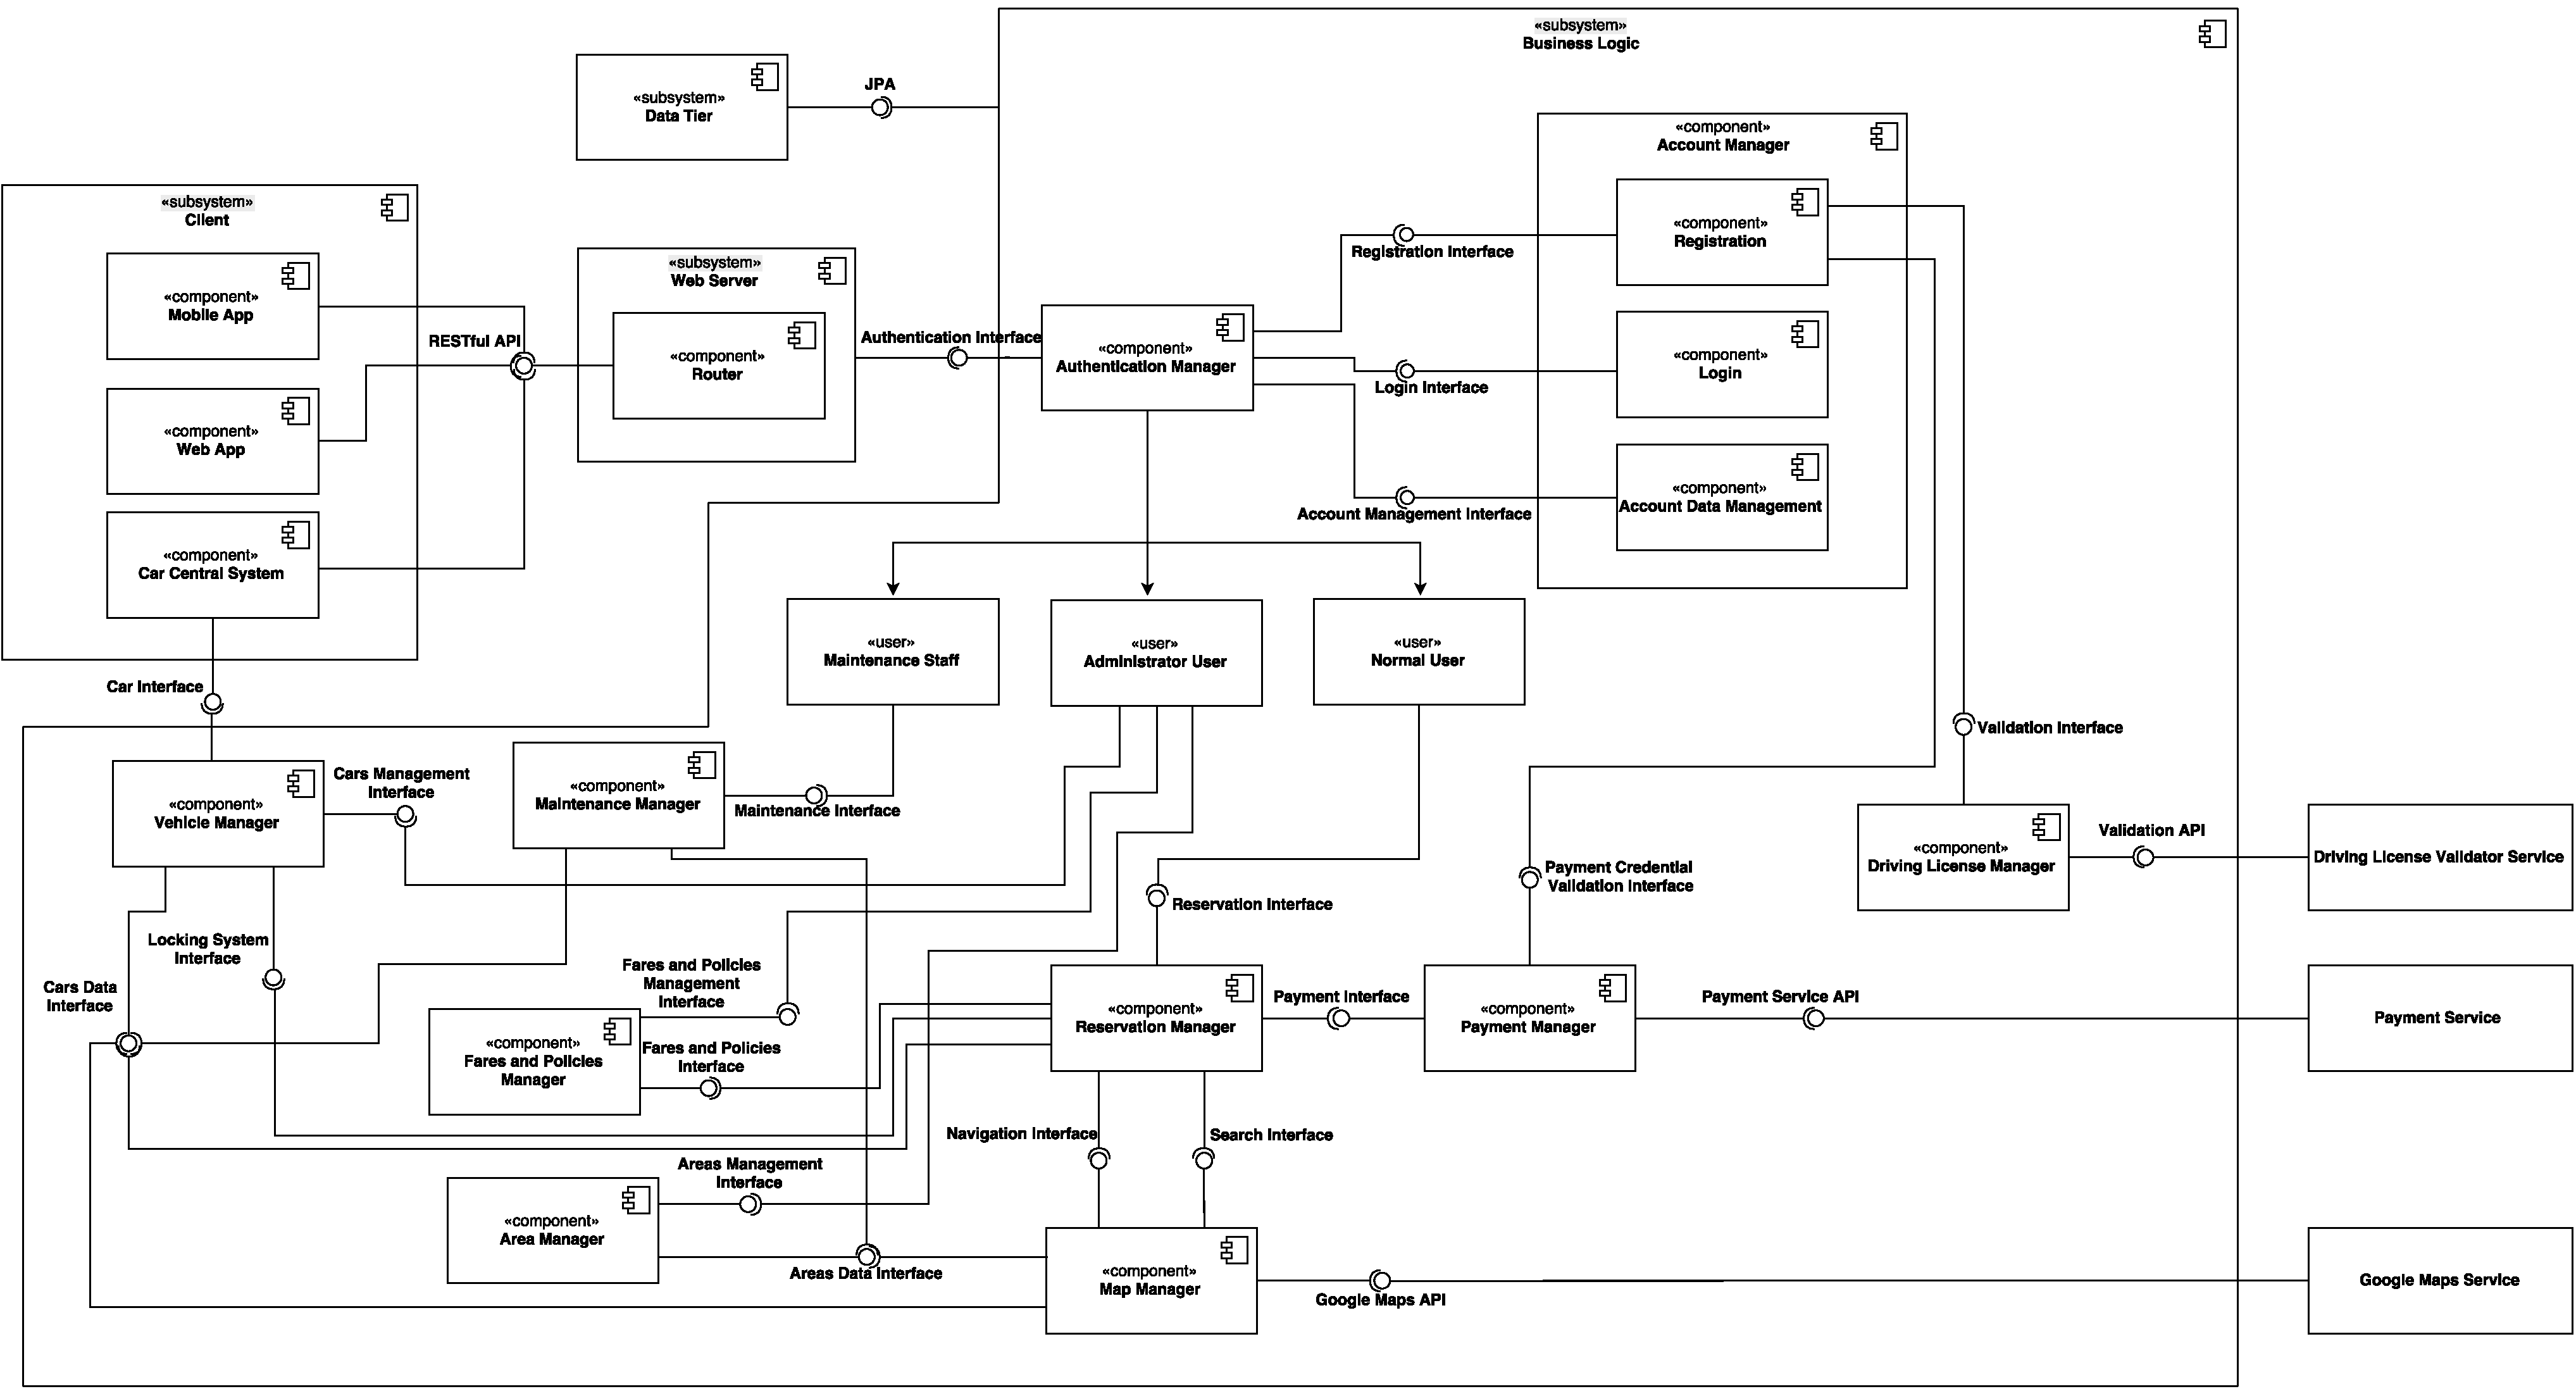
\includegraphics[width=350px]{../Datas/images/ComponentView.pdf}
	\caption{System component view}
	\label{fig:ComponentView}
\end{figure}

\subsubsection{Web Server and Authentication}

This image shows in detail the web server and the authentication component of
our system.

\begin{figure}[H]
	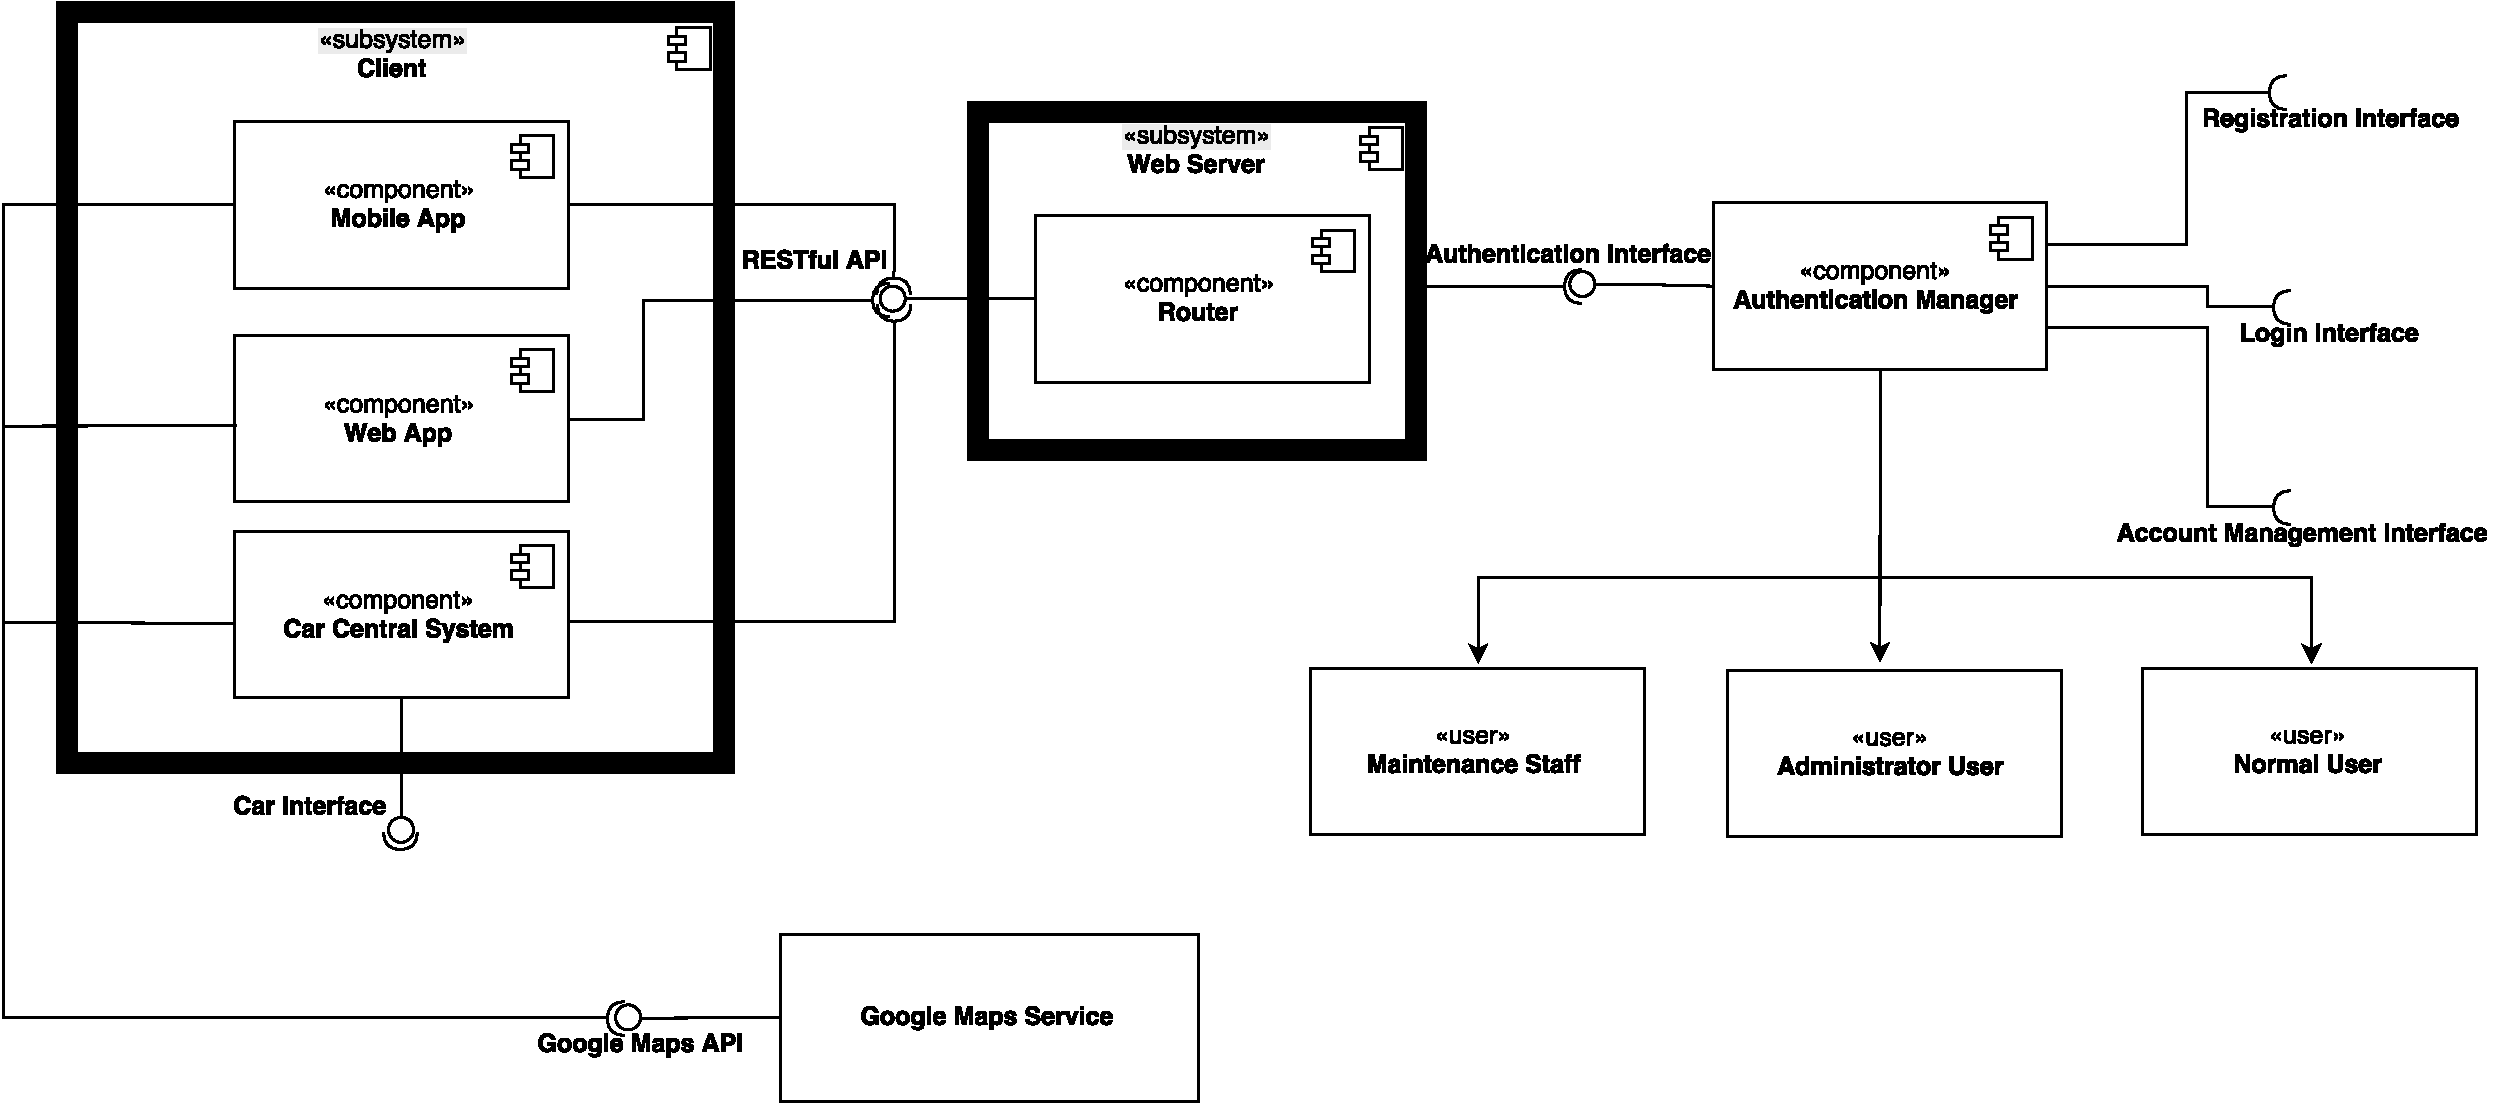
\includegraphics[width=350px]{../Datas/images/WebServerAndAuthenticationComponentView.pdf}
	\caption{Web Server and Authentication Component View}
	\label{fig:WebServerAndAuthenticationComponentView}
\end{figure}

\begin{itemize}
	\item \textbf{Mobile App}: This is the main client component, it's realized
														 starting from the web app and then adapted to the
														 mobile market using the PhoneGap framework.
	\item \textbf{Web App}: This is client application our users can use in a
													desktop eonvironment.
	\item \textbf{Router}: This represents the main component of the web server
												 used in our system that allows the clients to use our
												 application.
	\item \textbf{Authentication Manager}: This component is responsible for the
																				 authentication of our customers. Since
																				 we implemented our service following
																				 the REST guidelines we had to implement
																				 an authentication mechanism.
	\item \textbf{Normal User, Administrator User, Maintenance Staff}: These are
																				 the three categories of user recognized
																				 by our system.
\end{itemize}

\subsubsection{Account Manager}

This image presents a closer look at the account manager component, the
functions it provides and it's interactions with other components of the system.

\begin{figure}[H]
	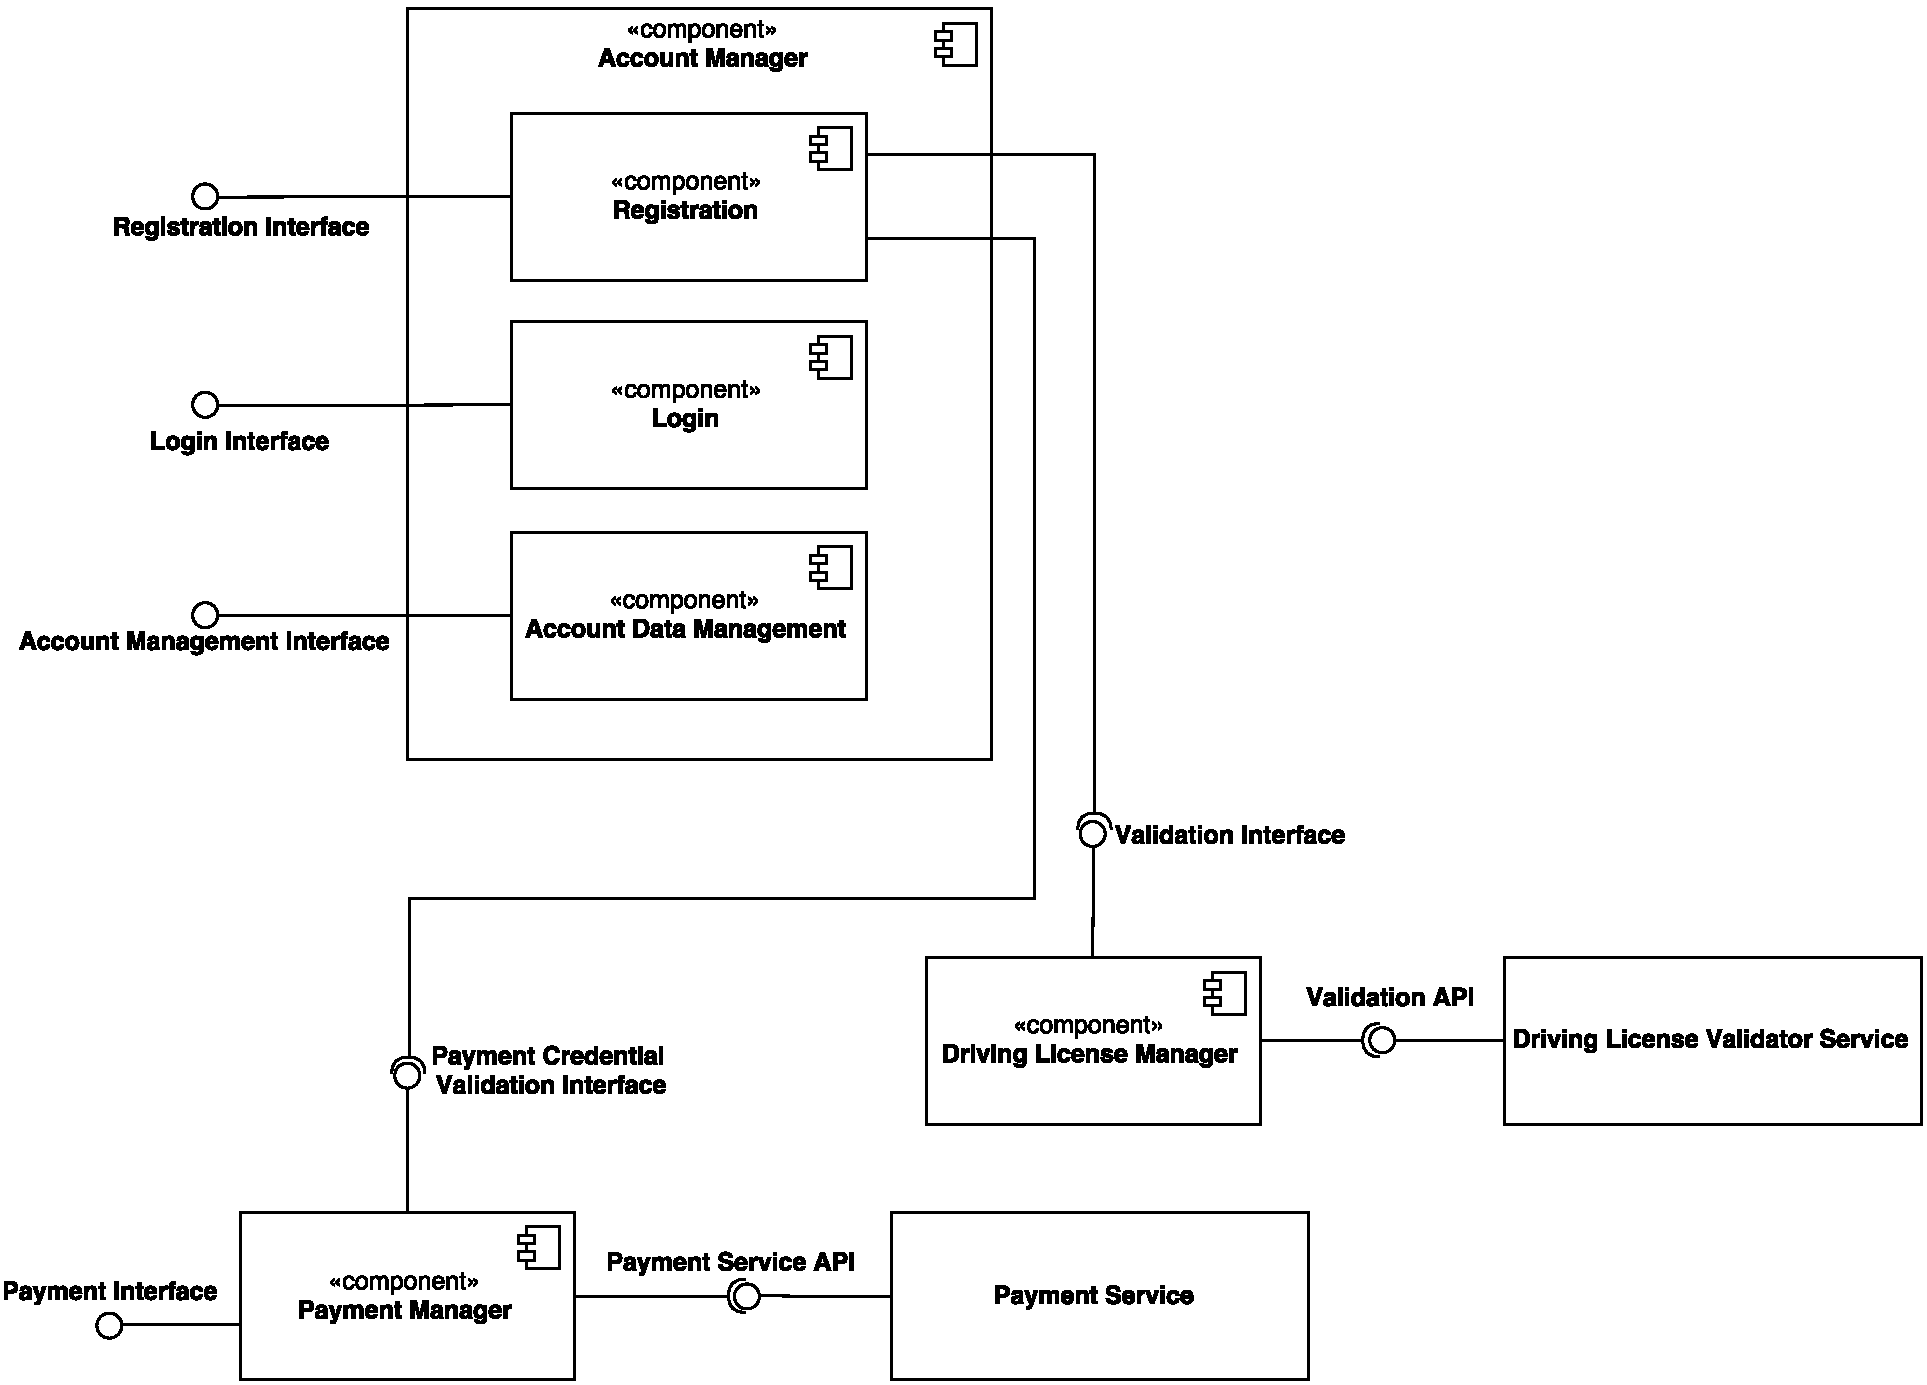
\includegraphics[width=350px]{../Datas/images/AuthenticationManagerComponentView.pdf}
	\caption{Authentication manager component view}
	\label{fig:AuthenticationManagerComponentView}
\end{figure}

\begin{itemize}
	\item \textbf{Account Manager}: This is the component responsible for the
																	login, the registration and the management of
																	the account of each user. In fact this component
																	exposes the \textit{Registration Interface},
																	the \textit{Login Interface} and the
																	\textit{Account Management Interface}.
	\begin{itemize}
		\item \textbf{Registration}: This component takes care of the registration
																 of a user. In order to do so it uses the
																 \textit{Validation Interface} exposed by the
																 \textit{Driving License Manager} to verify the
																 authenticity of the user's driving license, and
																 the \textit{Payment Credential Validation Interface}
																 exposed by the \textit{Payment Manager} to
																 check the payment informations submitted by the
																 user.
		\item \textbf{Login}: This is the component used when a user is logging into
													the system.
		\item \textbf{Account Data Management}: This component allows the user to
																						change the informations associated
																						with his account.
	\end{itemize}
	\item \textbf{Driving License Manager}: This component verifies whether or not
	 																				the driving license submitted by the
																					user is valid, to do so it uses the
																					\textit{Validation API} interface
																					exposed by the
																					\textit{Driving License Validator Service}.
	\item \textbf{Payment Manager}: This is the component that handles the
																	payments and checks if the data submitted by
																	the user during the registration process are
																	related to a valid payment method.
	\item \textbf{Driving License Validator Service}: \textit{IDCHECK.IO} is the
																	external service we decided to use in order to
																	check the driving license of the users that
																	want to register in our system.
	\item \textbf{Payment Service}: \textit{LevelUp} is the external service on
																	which our system relies on in order to handle
																	the payments.
\end{itemize}

\subsubsection{Car System}

This image presents the car system, it's interaction with the business logic and
it's subcomponents.

\begin{figure}[H]
	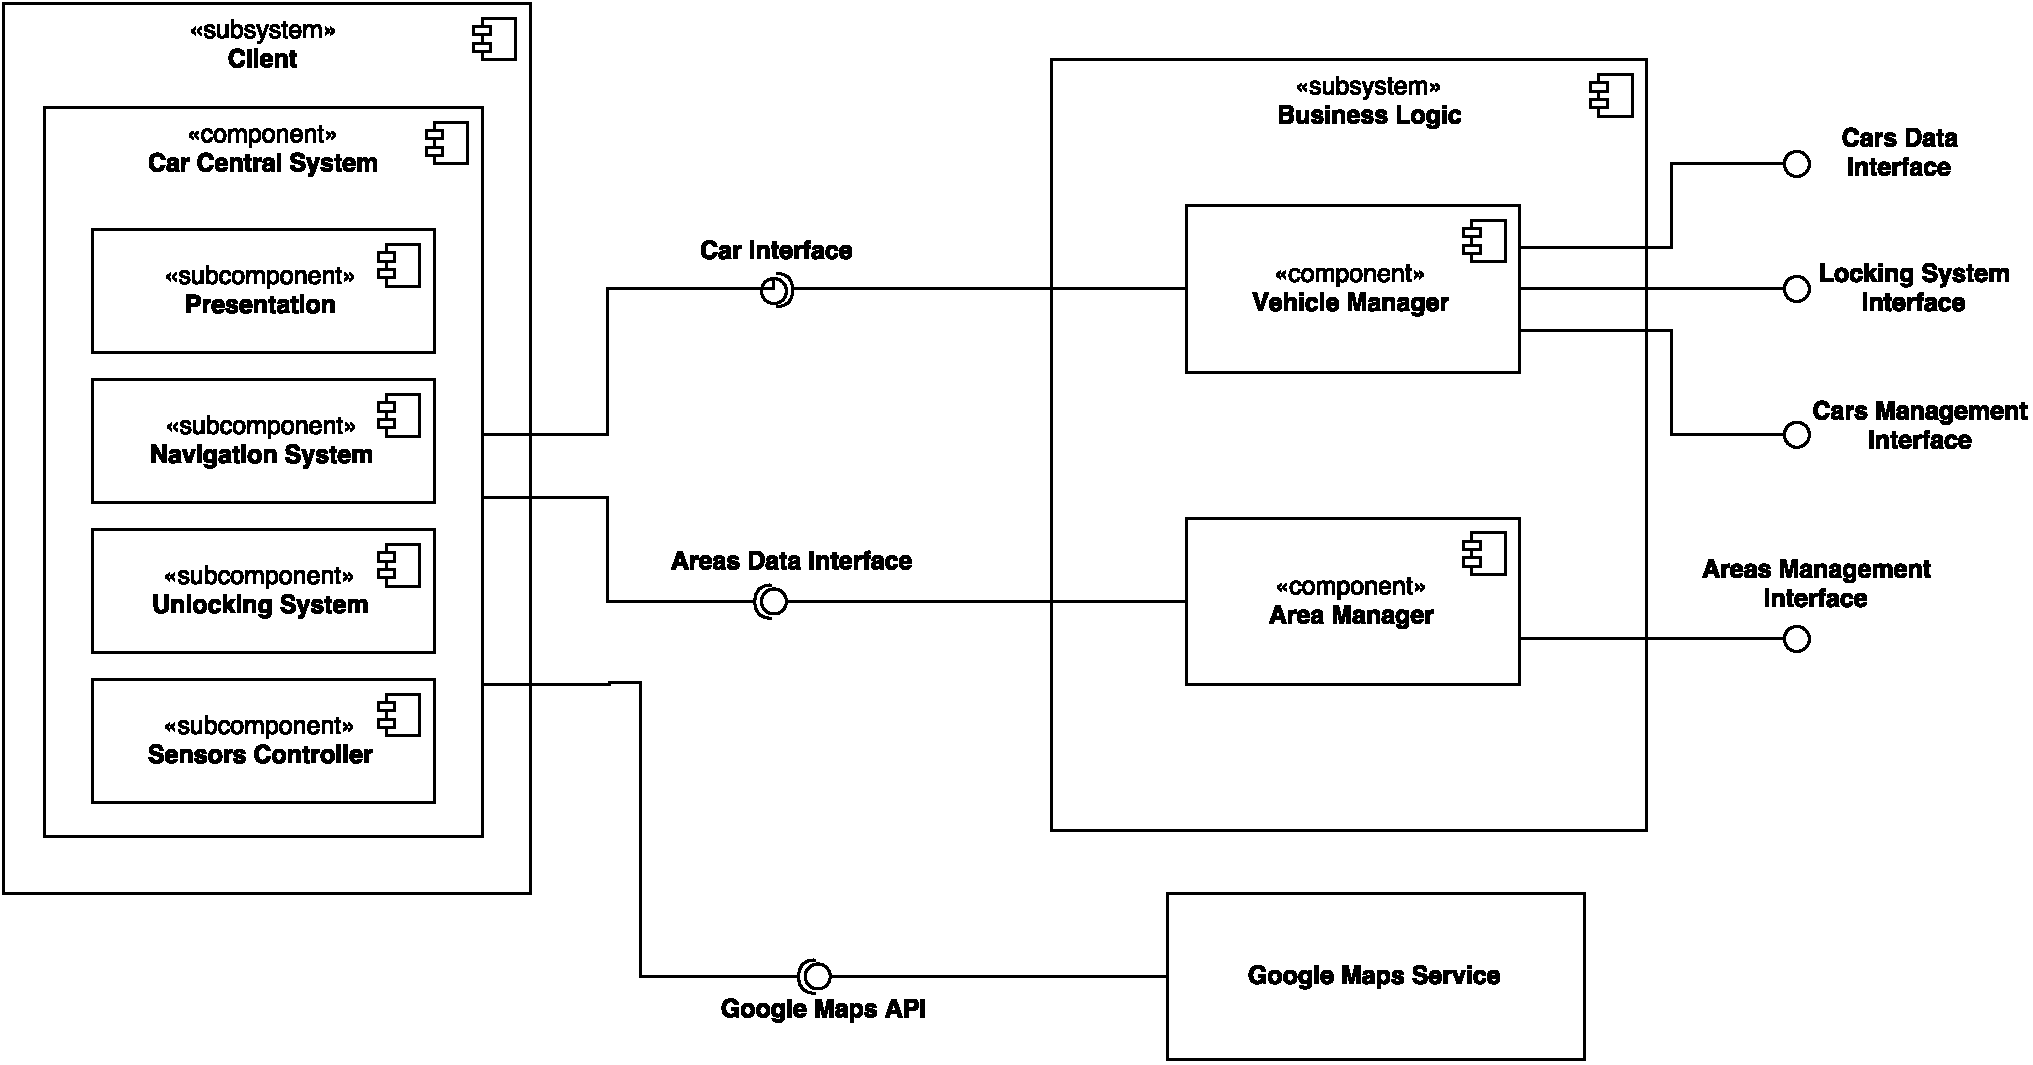
\includegraphics[width=350px]{../Datas/images/CarComponentView.pdf}
	\caption{Car system component view}
	\label{fig:CarSystemComponentView}
\end{figure}

\begin{itemize}
	\item \textbf{Car Central System}: This is the main component of each car,
																		 it is composed of different subcomponents
																		 each one performing a crucial task for the
																		 system.

	\begin{itemize}
	\item \textbf{Presentation}: This is the subcomponent responsible for the
															 interface shown to the user on the on-board touch
															 display.
	\item \textbf{Navigation System}: This subcomponent provides the user with a
																		step-by-step navigation he can use to reach
																		his destination. It recovers the
																		informations about the parking areas
																		position though the datas given by the
																		\textit{Areas Data Interface}.
	\item \textbf{Unlocking System}: This subcomponent communicates with the
																	 digital keyboard installed on the car's door
																	 allowing the user to lock and unlock the car.
	\item \textbf{Sensors Controller}: This is the subcomponent that collects all
																		 the datas coming from the different sensors
																		 placed on the car. (e.g. Battery Charge, GPS
																		 position,...)

	\end{itemize}

	\item \textbf{Vehicle Manager}: This component interacts with the car through
																	the \textit{Car Interface} exposed by the
																	\textit{Car Central System}. This is the
																	component inside the application server that
																	keeps all the informations about the cars and
																	is used for all the interactions with them.
	\item \textbf{Area Manager}: This is the component that controls all the
															 parking areas of the company, it exposes the
															 \textit{Areas Data Interface} that the
															 \textit{Car Central System} uses to access the
															 informations about the position of the parking
															 areas, and the
															 \textit{Areas Management Interface} that allows
															 an administrator to modify every aspect of the
															 parking areas.
\end{itemize}


\subsubsection{Normal User}

This image provides an overview of the functionalities that are specifically
available to a normal user of our system.

\begin{figure}[H]
	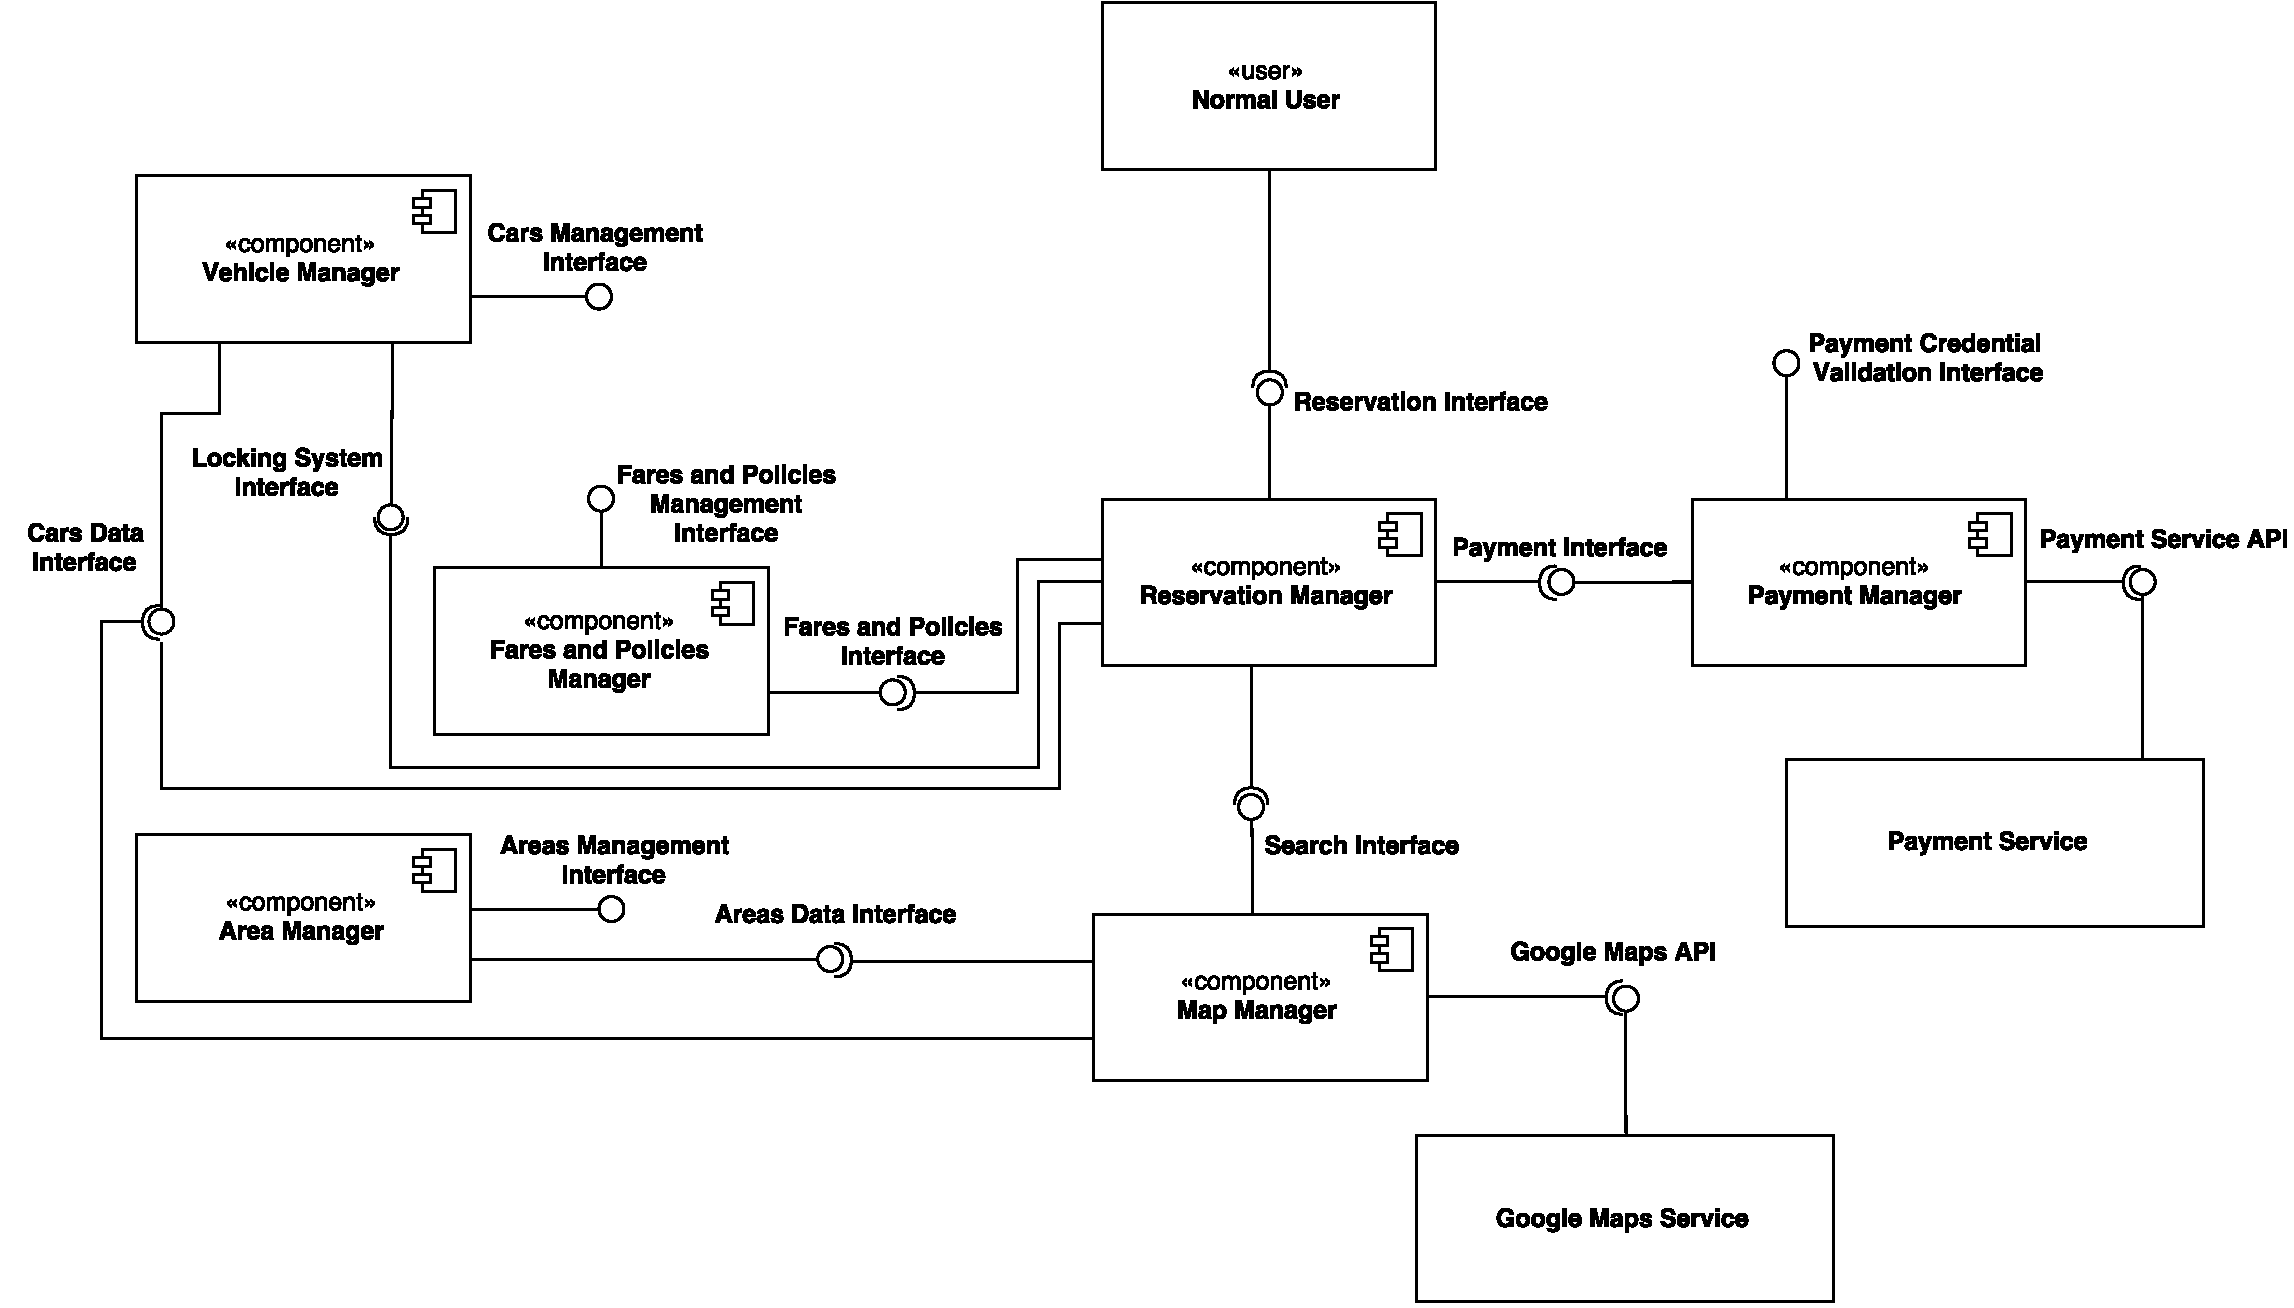
\includegraphics[width=350px]{../Datas/images/NormalUserComponentView.pdf}
	\caption{User Component View}
	\label{fig:UserComponentView}
\end{figure}

\begin{itemize}
\item \textbf{Reservation Manager}: This is the component that manages all the
																		aspects of a reservation. In order to do so
																		it has to communicate with different
																		components of our system.
\item \textbf{Fares and Policies Manager}: This is the component that handles
																					 all the fares and policies of the
																					 company. It can be accessed
\item \textbf{Map Manager}: This is the component responsible for all the
														maps related functionalities present in the system.
\item \textbf{Google Maps Service}: Google Maps is the service we decided to use
																		to address our need of a reliable and
																		functional service to handle a map.
\end {itemize}

\subsubsection{Maintenance User}

This image focuses on the maintenace user, showing the components it can access
and it's funtionalities in our system.

\begin{figure}[H]
	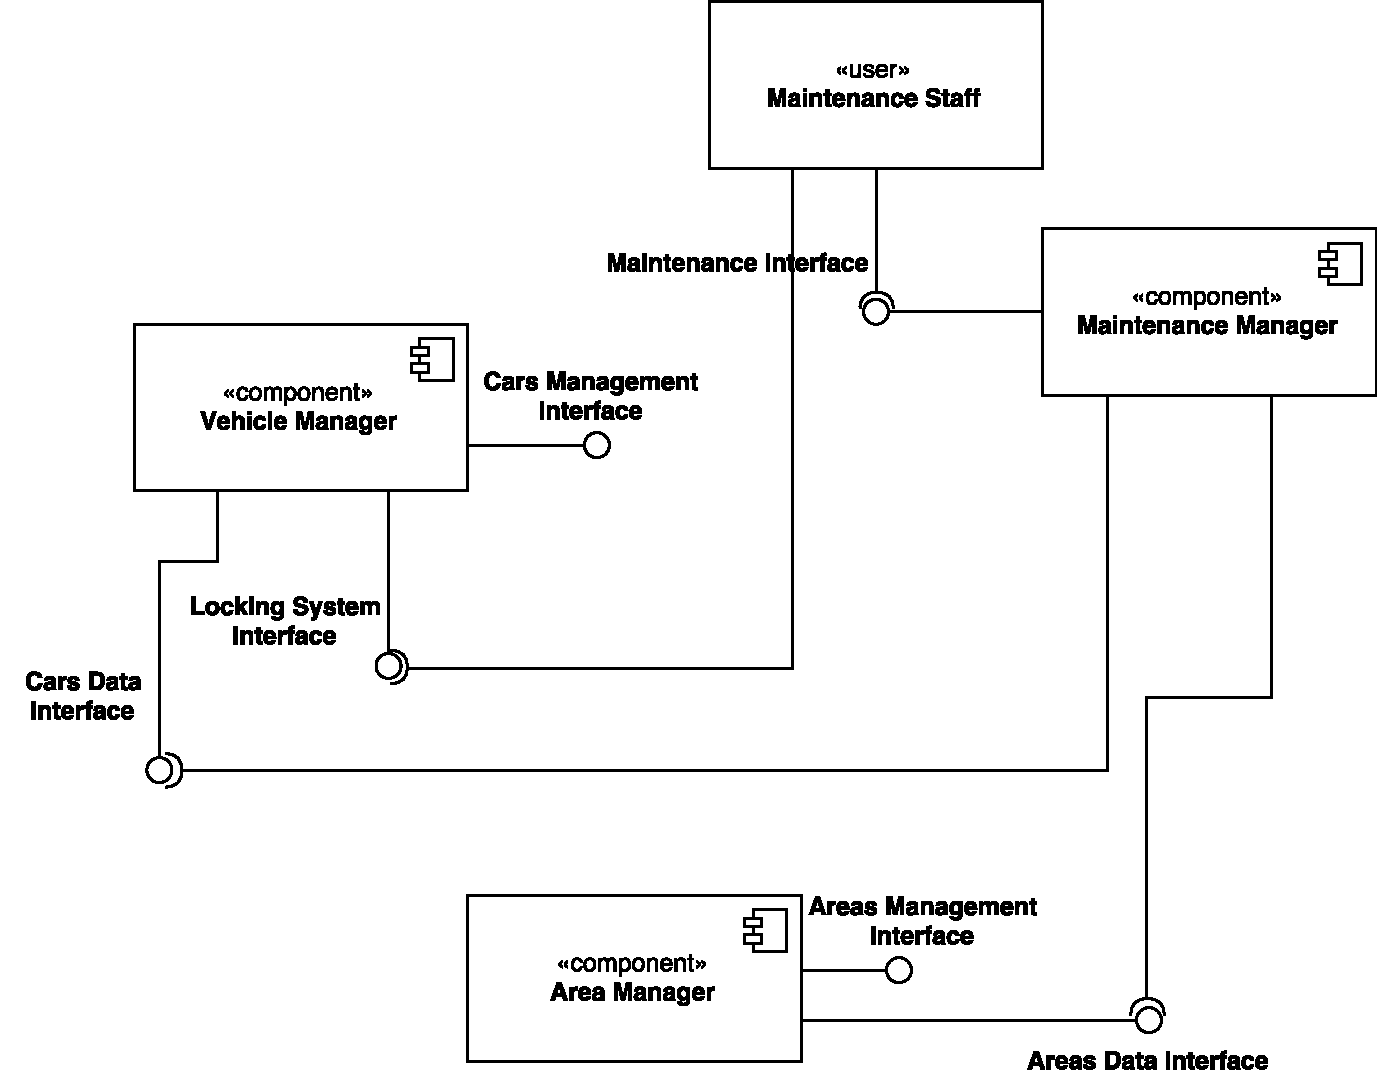
\includegraphics[width=350px]{../Datas/images/MaintenanceUserComponentView.pdf}
	\caption{Maintenance User Component View}
	\label{fig:MaintenanceUserComponentView}
\end{figure}

\begin{itemize}
\item \textbf{Maintenance Manager}: This component looks for any kind of
																		problem regarding cars and parking areas so
																		that the maintanace staff can promptly take
																		action in order to resolve that problem.
\end {itemize}

\subsubsection{Administrator User}

This image shows the functionalities exclusively available to an administrator
user of our system.

\begin{figure}[H]
	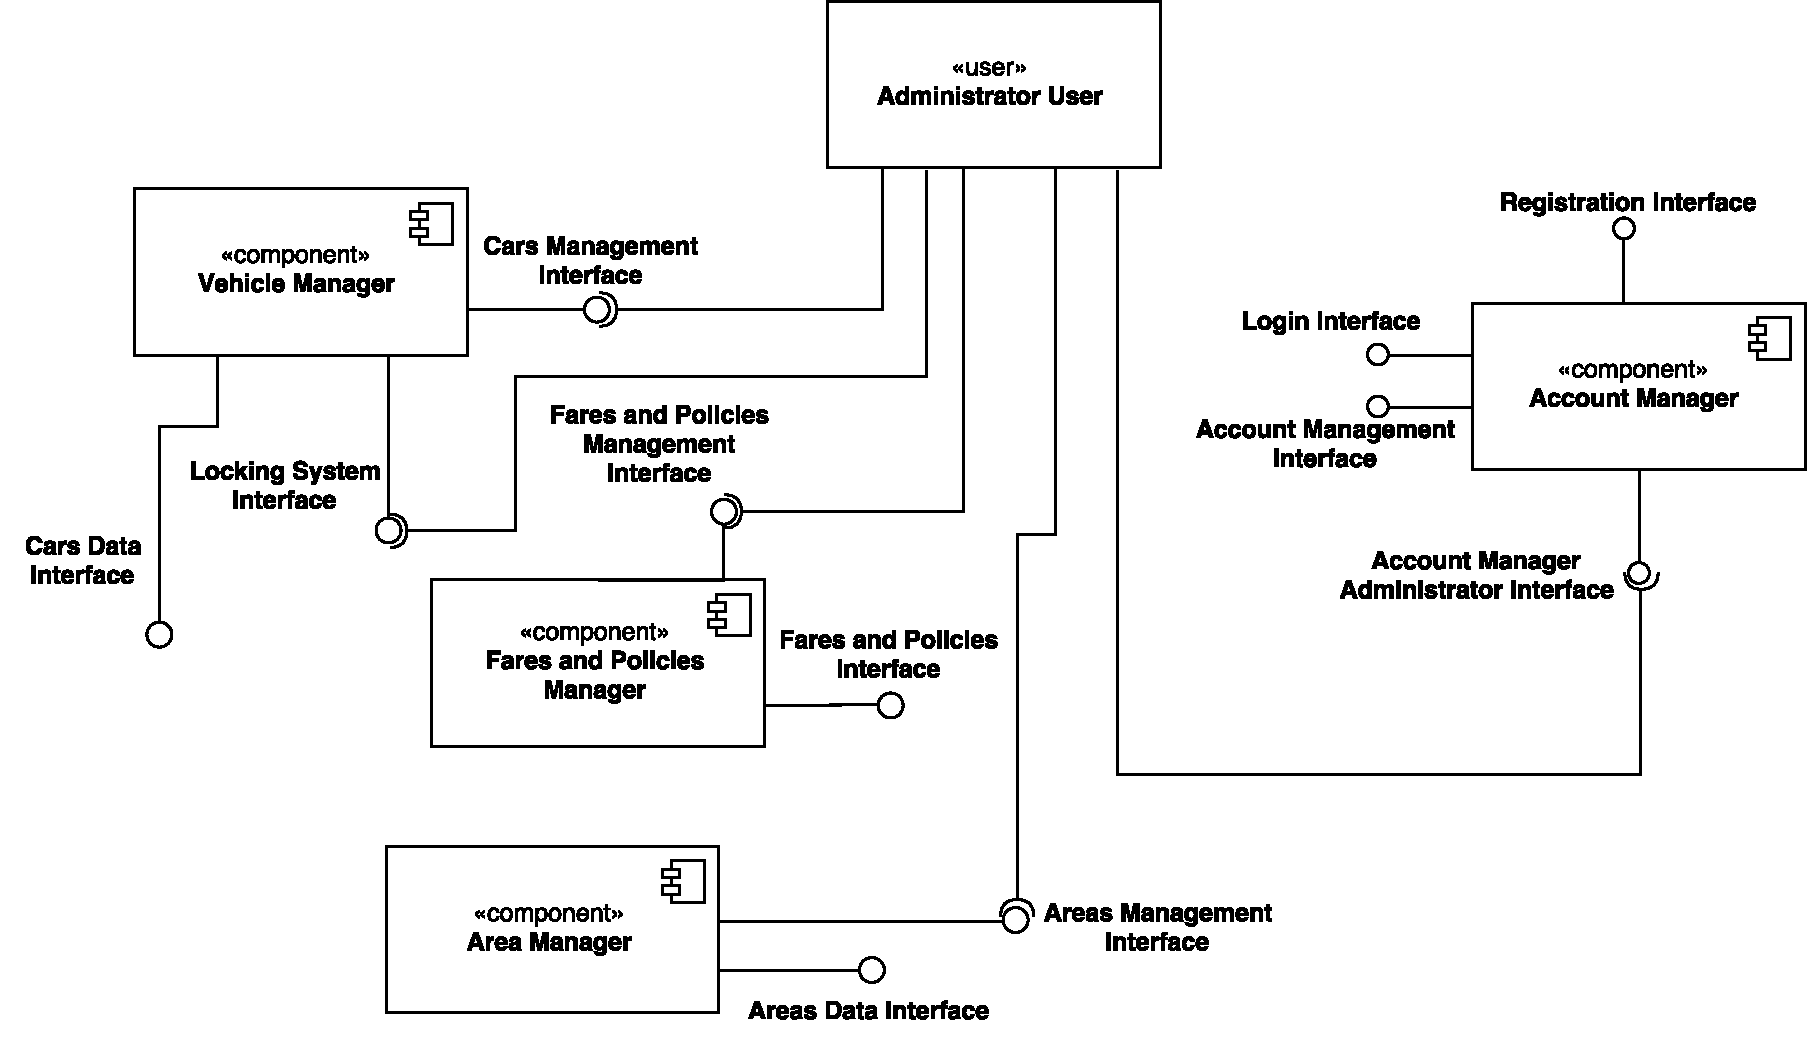
\includegraphics[width=350px]{../Datas/images/AdministratorComponentView.pdf}
	\caption{Administrator Component View}
	\label{fig:AdministratorComponentView}
\end{figure}

\newpage
